\documentclass[border=4pt]{standalone}
\usepackage{amsmath,amssymb}
\usepackage{tikz}
\usetikzlibrary{arrows.meta,decorations.pathreplacing}
\begin{document}
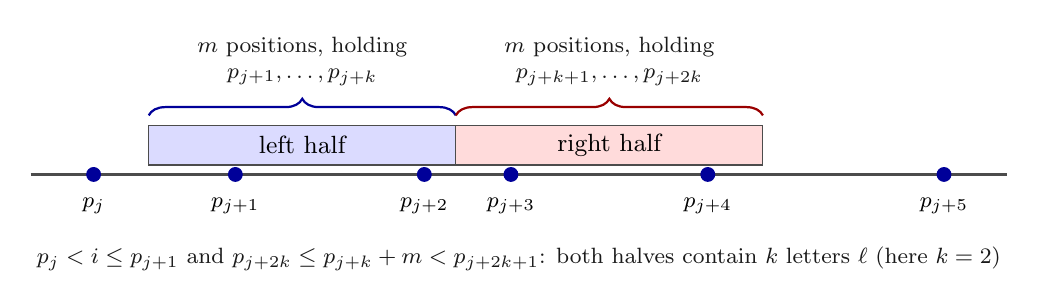
\begin{tikzpicture}[
  >={Stealth[length=2.2mm]},
  note/.style={font=\footnotesize,gray!20!black,align=center},
  occ/.style={circle,fill=blue!60!black,inner sep=1.9pt},
  br/.style={decorate,decoration={brace,amplitude=6pt},thick},
  brm/.style={decorate,decoration={brace,amplitude=6pt,mirror},thick}]
  % occurrences of the letter l, k = 2: p_j, ..., p_{j+5}
  \def\pj{0.0} \def\pa{1.8} \def\pb{4.2} \def\pc{5.3} \def\pd{7.8} \def\pe{10.8}
  \draw[gray!60!black,thick] (-0.8,0) -- (11.6,0);
  \foreach \x/\lab in {\pj/{p_j},\pa/{p_{j+1}},\pb/{p_{j+2}},\pc/{p_{j+3}},\pd/{p_{j+4}},\pe/{p_{j+5}}} {
    \node[occ] at (\x,0) {};
    \node[font=\footnotesize,below=5pt] at (\x,0) {$\lab$};
  }
  % the square: left half (i .. p_{j+2}], right half (p_{j+2} .. p_{j+2}+m]
  \def\i{0.7}
  \def\h{4.6}
  \def\m{3.9}
  \fill[blue!14] (\i,0.12) rectangle (\h,0.62);
  \fill[red!14] (\h,0.12) rectangle ({\h+\m},0.62);
  \draw[gray!60!black] (\i,0.12) rectangle ({\h+\m},0.62);
  \draw[gray!60!black] (\h,0.12) -- (\h,0.62);
  \node[font=\small] at ({(\i+\h)/2},0.37) {left half};
  \node[font=\small] at ({\h+\m/2},0.37) {right half};
  \draw[br,blue!60!black] (\i,0.75) -- node[above=7pt,note]{$m$ positions, holding\\ $p_{j+1},\dots,p_{j+k}$} (\h,0.75);
  \draw[br,red!60!black] (\h,0.75) -- node[above=7pt,note]{$m$ positions, holding\\ $p_{j+k+1},\dots,p_{j+2k}$} ({\h+\m},0.75);
  \node[note,anchor=north] at (5.4,-0.8)
    {$p_j<i\le p_{j+1}$ and $p_{j+2k}\le p_{j+k}+m<p_{j+2k+1}$: both halves contain $k$ letters $\ell$ (here $k=2$)};
\end{tikzpicture}
\end{document}
